\subsection{Implementation and Results}

We can demonstrate an autoencoder for cryptography by attempting to encrypt binary representation of characters. Previous studies show the viability of such autoencoders for 8-bit ASCII characters \cite{icaart20}, so we will expand on this example and do it for Unicode characters.

Firstly, the training data is determined by generating all Unicode characters, for which we need at least 21 bits. If we define the training data as $X$, then it can be defined as follows:

\begin{equation}
    X = \{x \in \{0,1\}^{21} \mid x = \text{bin}(i), i \in [0, 1114111]\}
\end{equation}

As it was discussed previously, the output of the neural network will be of the same dimension as its input. The depth of the neural network depends on the specific application, and the complexity of the system. Many sources suggest that a hidden encoder layer and a hidden decoder layer are sufficient for general purposes \cite{autoencoder2}. In this case, we will use a hidden layer of 32 neurons for both the encoder and the decoder. The activation function for the hidden layers will be the rectified linear unit (ReLU) function, and the output layer will use the sigmoid function. The sigmoid function is used because it is a good choice for binary classification problems. The ReLU function is used because it is a good choice for hidden layers in general, and it is the most common activation function for autoencoders \cite{autoencoder3}. The loss function to optimize is binary cross entropy, due to the binary nature of the input and output data. The optimizer used is the Adam optimizer, which is a popular choice for general purpose neural networks. The autoencoder will be trained for 50 epochs.

Since the encoding dimension will represent the characters, it is the most important parameter of the autoencoder. To determine an appropriate encoding dimension, we may train multiple autoencoders with different encoding dimensions, and compare their performance. The performance of the autoencoder will be measured by the percentage of characters that are correctly reconstructed. The encoding dimensions to be tested are 8, 12, and 16.

The results of reconstruction efficiency for the different encoding dimensions are shown in \autoref{tab:results}. The results show that the autoencoder with an encoding dimension of 16 is the most efficient, with a reconstruction efficiency of 100\%. This means that using this autoencoder we could be capable of encrypting and decrypting Unicode characters in a lossless manner. The other encoding dimensions do not reach 100\% efficiency, therefore they are not suitable for this application.

\begin{table}[h]
    \centering
    \begin{tabular}{|c|c|c|}
        \hline
        Encoding Dimension & Reconstruction Efficiency & Final Loss Value      \\
        \hline
        8                  & 4.43\%                    & 0.1715                \\
        12                 & 33.83\%                   & 0.0794                \\
        16                 & 100\%                     & 7.6340$\times10^{-5}$ \\
        \hline
    \end{tabular}
    \caption{Reconstruction efficiency for different encoding dimensions}
    \label{tab:results}
\end{table}

We may assume that encoding dimensions bigger than 16 will also have 100\% reconstruction efficiency, but they will be more computationally expensive. Therefore, we can conclude that the best autoencoder for this application is the one with an encoding dimension of 16. The system can be tested by encoding and decoding text with Unicode characters, as it is shown in \autoref{fig:unicode}. In the figure we can see that the autoencoder is capable of reconstructing all characters without error. A preview of the first two character encryptions is shown too.

\begin{figure}[h]
    \centering
    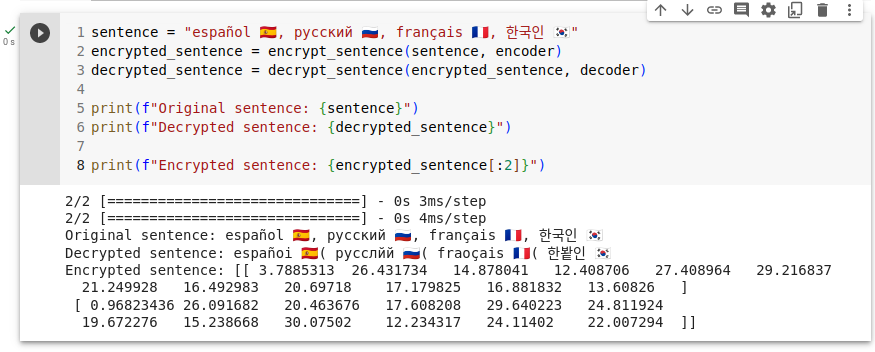
\includegraphics[width=\textwidth]{img/unicode.png}
    \caption{Encoding and decoding Unicode characters.}
    \label{fig:unicode}
\end{figure}

\subsection{Discussion}

Although the network is capable of reconstructing all characters without error, one of the issues is the transmission of the encoded messages. The best performing model has a 16-dimensional code, which means that the encrypted characters consists of 16 neuron activations, which are in turn, 16 floating point numbers. This means that the encrypted message is more than 20 times larger than the original message. This is a significant increase in size, and it is not suitable for most applications. However, it is possible to reduce the size of the encoded message by using a smaller encoding dimension, at the cost of reconstruction efficiency.

Of course, another option is to utilize a different activation function for the encoding layer, so that it can be discretized more easily, and thus, transmitted. However, this would require a different loss function, and a deeper neural network, since it would be more difficult to reconstruct the original message. This would also increase the computational complexity of the system, which is not desirable.

Nonetheless, this example shows that autoencoders can be used for cryptography, and that they can be used to encrypt and decrypt messages without error. This shows that autoencoders can be used for lossless encryption, although it would take a more sophisticated system to achieve lossless encryption with a reasonable message size.

Furthermore, the complexity of AES, the most popular encryption algorithm, is $O(n)$, where $n$ is the number of bits in the message \cite{aes}. This means that the complexity of AES is linear with respect to the message size. On the other hand, the complexity of the autoencoder is $O(n^2)$, where $n$ is the number of neurons in the network. This means that the complexity of the autoencoder is quadratic with respect to the message size.
